\documentclass[11pt]{article}
\renewcommand{\arraystretch}{1.5} % Default value: 1
\usepackage{sectsty}
\allsectionsfont{\color{blue}\fontfamily{lmss}\selectfont}
\usepackage{fontspec}
\setmainfont{XCharter}

\usepackage{listings}
\lstset{
basicstyle=\small\ttfamily,
tabsize=8,
columns=flexible,
breaklines=true,
frame=tb,
rulecolor=\color[rgb]{0.8,0.8,0.7},
backgroundcolor=\color[rgb]{1,1,0.91},
postbreak=\raisebox{0ex}[0ex][0ex]{\ensuremath{\color{red}\hookrightarrow\space}}
}
\usepackage{fontawesome}


\usepackage{mdframed}
\newmdenv[
  backgroundcolor=gray,
  fontcolor=white,
  nobreak=true,
]{terminalinput}



\usepackage{parskip}




    \usepackage[T1]{fontenc}
    % Nicer default font than Computer Modern for most use cases
    \usepackage{palatino}

    % Basic figure setup, for now with no caption control since it's done
    % automatically by Pandoc (which extracts ![](path) syntax from Markdown).
    \usepackage{graphicx}
    % We will generate all images so they have a width \maxwidth. This means
    % that they will get their normal width if they fit onto the page, but
    % are scaled down if they would overflow the margins.
    \makeatletter
    \def\maxwidth{\ifdim\Gin@nat@width>\linewidth\linewidth
    \else\Gin@nat@width\fi}
    \makeatother
    \let\Oldincludegraphics\includegraphics
    % Set max figure width to be 80% of text width, for now hardcoded.
\renewcommand{\includegraphics}[1]{\Oldincludegraphics[width=.8\maxwidth, height=.55\textheight, keepaspectratio]{#1}}
    % Ensure that by default, figures have no caption (until we provide a
    % proper Figure object with a Caption API and a way to capture that
    % in the conversion process - todo).
    \usepackage{caption}
    \DeclareCaptionLabelFormat{nolabel}{}
    \captionsetup{labelformat=nolabel, textfont=bf}

    \usepackage{adjustbox} % Used to constrain images to a maximum size
    \usepackage{xcolor} % Allow colors to be defined
    \usepackage{enumerate} % Needed for markdown enumerations to work
    \usepackage{geometry} % Used to adjust the document margins
    \usepackage{amsmath} % Equations
    \usepackage{amssymb} % Equations
    \usepackage{textcomp} % defines textquotesingle
    % Hack from http://tex.stackexchange.com/a/47451/13684:
    \AtBeginDocument{%
        \def\PYZsq{\textquotesingle}% Upright quotes in Pygmentized code
    }
    \usepackage{upquote} % Upright quotes for verbatim code
    \usepackage{eurosym} % defines \euro
    \usepackage[mathletters]{ucs} % Extended unicode (utf-8) support
    \usepackage[utf8x]{inputenc} % Allow utf-8 characters in the tex document
    \usepackage{fancyvrb} % verbatim replacement that allows latex
    \usepackage{grffile} % extends the file name processing of package graphics
                         % to support a larger range
    % The hyperref package gives us a pdf with properly built
    % internal navigation ('pdf bookmarks' for the table of contents,
    % internal cross-reference links, web links for URLs, etc.)
    \usepackage{hyperref}
    \usepackage{longtable} % longtable support required by pandoc >1.10
    \usepackage{booktabs}  % table support for pandoc > 1.12.2
    \usepackage[normalem]{ulem} % ulem is needed to support strikethroughs (\sout)
                                % normalem makes italics be italics, not underlines




    % Colors for the hyperref package
    \definecolor{urlcolor}{rgb}{0,.145,.698}
    \definecolor{linkcolor}{rgb}{.71,0.21,0.01}
    \definecolor{citecolor}{rgb}{.12,.54,.11}

    % ANSI colors
    \definecolor{ansi-black}{HTML}{3E424D}
    \definecolor{ansi-black-intense}{HTML}{282C36}
    \definecolor{ansi-red}{HTML}{E75C58}
    \definecolor{ansi-red-intense}{HTML}{B22B31}
    \definecolor{ansi-green}{HTML}{00A250}
    \definecolor{ansi-green-intense}{HTML}{007427}
    \definecolor{ansi-yellow}{HTML}{DDB62B}
    \definecolor{ansi-yellow-intense}{HTML}{B27D12}
    \definecolor{ansi-blue}{HTML}{208FFB}
    \definecolor{ansi-blue-intense}{HTML}{0065CA}
    \definecolor{ansi-magenta}{HTML}{D160C4}
    \definecolor{ansi-magenta-intense}{HTML}{A03196}
    \definecolor{ansi-cyan}{HTML}{60C6C8}
    \definecolor{ansi-cyan-intense}{HTML}{258F8F}
    \definecolor{ansi-white}{HTML}{C5C1B4}
    \definecolor{ansi-white-intense}{HTML}{A1A6B2}

    % commands and environments needed by pandoc snippets
    % extracted from the output of `pandoc -s`
    \providecommand{\tightlist}{%
      \setlength{\itemsep}{0pt}\setlength{\parskip}{0pt}}
    \DefineVerbatimEnvironment{Highlighting}{Verbatim}{commandchars=\\\{\}}
    % Add ',fontsize=\small' for more characters per line
    \newenvironment{Shaded}{}{}
    \newcommand{\KeywordTok}[1]{\textcolor[rgb]{0.00,0.44,0.13}{\textbf{{#1}}}}
    \newcommand{\DataTypeTok}[1]{\textcolor[rgb]{0.56,0.13,0.00}{{#1}}}
    \newcommand{\DecValTok}[1]{\textcolor[rgb]{0.25,0.63,0.44}{{#1}}}
    \newcommand{\BaseNTok}[1]{\textcolor[rgb]{0.25,0.63,0.44}{{#1}}}
    \newcommand{\FloatTok}[1]{\textcolor[rgb]{0.25,0.63,0.44}{{#1}}}
    \newcommand{\CharTok}[1]{\textcolor[rgb]{0.25,0.44,0.63}{{#1}}}
    \newcommand{\StringTok}[1]{\textcolor[rgb]{0.25,0.44,0.63}{{#1}}}
    \newcommand{\CommentTok}[1]{\textcolor[rgb]{0.38,0.63,0.69}{\textit{{#1}}}}
    \newcommand{\OtherTok}[1]{\textcolor[rgb]{0.00,0.44,0.13}{{#1}}}
    \newcommand{\AlertTok}[1]{\textcolor[rgb]{1.00,0.00,0.00}{\textbf{{#1}}}}
    \newcommand{\FunctionTok}[1]{\textcolor[rgb]{0.02,0.16,0.49}{{#1}}}
    \newcommand{\RegionMarkerTok}[1]{{#1}}
    \newcommand{\ErrorTok}[1]{\textcolor[rgb]{1.00,0.00,0.00}{\textbf{{#1}}}}
    \newcommand{\NormalTok}[1]{{#1}}

    % Additional commands for more recent versions of Pandoc
    \newcommand{\ConstantTok}[1]{\textcolor[rgb]{0.53,0.00,0.00}{{#1}}}
    \newcommand{\SpecialCharTok}[1]{\textcolor[rgb]{0.25,0.44,0.63}{{#1}}}
    \newcommand{\VerbatimStringTok}[1]{\textcolor[rgb]{0.25,0.44,0.63}{{#1}}}
    \newcommand{\SpecialStringTok}[1]{\textcolor[rgb]{0.73,0.40,0.53}{{#1}}}
    \newcommand{\ImportTok}[1]{{#1}}
    \newcommand{\DocumentationTok}[1]{\textcolor[rgb]{0.73,0.13,0.13}{\textit{{#1}}}}
    \newcommand{\AnnotationTok}[1]{\textcolor[rgb]{0.38,0.63,0.69}{\textbf{\textit{{#1}}}}}
    \newcommand{\CommentVarTok}[1]{\textcolor[rgb]{0.38,0.63,0.69}{\textbf{\textit{{#1}}}}}
    \newcommand{\VariableTok}[1]{\textcolor[rgb]{0.10,0.09,0.49}{{#1}}}
    \newcommand{\ControlFlowTok}[1]{\textcolor[rgb]{0.00,0.44,0.13}{\textbf{{#1}}}}
    \newcommand{\OperatorTok}[1]{\textcolor[rgb]{0.40,0.40,0.40}{{#1}}}
    \newcommand{\BuiltInTok}[1]{{#1}}
    \newcommand{\ExtensionTok}[1]{{#1}}
    \newcommand{\PreprocessorTok}[1]{\textcolor[rgb]{0.74,0.48,0.00}{{#1}}}
    \newcommand{\AttributeTok}[1]{\textcolor[rgb]{0.49,0.56,0.16}{{#1}}}
    \newcommand{\InformationTok}[1]{\textcolor[rgb]{0.38,0.63,0.69}{\textbf{\textit{{#1}}}}}
    \newcommand{\WarningTok}[1]{\textcolor[rgb]{0.38,0.63,0.69}{\textbf{\textit{{#1}}}}}


    % Define a nice break command that doesn't care if a line doesn't already
    % exist.
    \def\br{\hspace*{\fill} \\* }
    % Math Jax compatability definitions
    \def\gt{>}
    \def\lt{<}
    % Document parameters
    \title{index}




    % Pygments definitions

\makeatletter
\def\PY@reset{\let\PY@it=\relax \let\PY@bf=\relax%
    \let\PY@ul=\relax \let\PY@tc=\relax%
    \let\PY@bc=\relax \let\PY@ff=\relax}
\def\PY@tok#1{\csname PY@tok@#1\endcsname}
\def\PY@toks#1+{\ifx\relax#1\empty\else%
    \PY@tok{#1}\expandafter\PY@toks\fi}
\def\PY@do#1{\PY@bc{\PY@tc{\PY@ul{%
    \PY@it{\PY@bf{\PY@ff{#1}}}}}}}
\def\PY#1#2{\PY@reset\PY@toks#1+\relax+\PY@do{#2}}

\expandafter\def\csname PY@tok@w\endcsname{\def\PY@tc##1{\textcolor[rgb]{0.73,0.73,0.73}{##1}}}
\expandafter\def\csname PY@tok@c\endcsname{\let\PY@it=\textit\def\PY@tc##1{\textcolor[rgb]{0.25,0.50,0.50}{##1}}}
\expandafter\def\csname PY@tok@cp\endcsname{\def\PY@tc##1{\textcolor[rgb]{0.74,0.48,0.00}{##1}}}
\expandafter\def\csname PY@tok@k\endcsname{\let\PY@bf=\textbf\def\PY@tc##1{\textcolor[rgb]{0.00,0.50,0.00}{##1}}}
\expandafter\def\csname PY@tok@kp\endcsname{\def\PY@tc##1{\textcolor[rgb]{0.00,0.50,0.00}{##1}}}
\expandafter\def\csname PY@tok@kt\endcsname{\def\PY@tc##1{\textcolor[rgb]{0.69,0.00,0.25}{##1}}}
\expandafter\def\csname PY@tok@o\endcsname{\def\PY@tc##1{\textcolor[rgb]{0.40,0.40,0.40}{##1}}}
\expandafter\def\csname PY@tok@ow\endcsname{\let\PY@bf=\textbf\def\PY@tc##1{\textcolor[rgb]{0.67,0.13,1.00}{##1}}}
\expandafter\def\csname PY@tok@nb\endcsname{\def\PY@tc##1{\textcolor[rgb]{0.00,0.50,0.00}{##1}}}
\expandafter\def\csname PY@tok@nf\endcsname{\def\PY@tc##1{\textcolor[rgb]{0.00,0.00,1.00}{##1}}}
\expandafter\def\csname PY@tok@nc\endcsname{\let\PY@bf=\textbf\def\PY@tc##1{\textcolor[rgb]{0.00,0.00,1.00}{##1}}}
\expandafter\def\csname PY@tok@nn\endcsname{\let\PY@bf=\textbf\def\PY@tc##1{\textcolor[rgb]{0.00,0.00,1.00}{##1}}}
\expandafter\def\csname PY@tok@ne\endcsname{\let\PY@bf=\textbf\def\PY@tc##1{\textcolor[rgb]{0.82,0.25,0.23}{##1}}}
\expandafter\def\csname PY@tok@nv\endcsname{\def\PY@tc##1{\textcolor[rgb]{0.10,0.09,0.49}{##1}}}
\expandafter\def\csname PY@tok@no\endcsname{\def\PY@tc##1{\textcolor[rgb]{0.53,0.00,0.00}{##1}}}
\expandafter\def\csname PY@tok@nl\endcsname{\def\PY@tc##1{\textcolor[rgb]{0.63,0.63,0.00}{##1}}}
\expandafter\def\csname PY@tok@ni\endcsname{\let\PY@bf=\textbf\def\PY@tc##1{\textcolor[rgb]{0.60,0.60,0.60}{##1}}}
\expandafter\def\csname PY@tok@na\endcsname{\def\PY@tc##1{\textcolor[rgb]{0.49,0.56,0.16}{##1}}}
\expandafter\def\csname PY@tok@nt\endcsname{\let\PY@bf=\textbf\def\PY@tc##1{\textcolor[rgb]{0.00,0.50,0.00}{##1}}}
\expandafter\def\csname PY@tok@nd\endcsname{\def\PY@tc##1{\textcolor[rgb]{0.67,0.13,1.00}{##1}}}
\expandafter\def\csname PY@tok@s\endcsname{\def\PY@tc##1{\textcolor[rgb]{0.73,0.13,0.13}{##1}}}
\expandafter\def\csname PY@tok@sd\endcsname{\let\PY@it=\textit\def\PY@tc##1{\textcolor[rgb]{0.73,0.13,0.13}{##1}}}
\expandafter\def\csname PY@tok@si\endcsname{\let\PY@bf=\textbf\def\PY@tc##1{\textcolor[rgb]{0.73,0.40,0.53}{##1}}}
\expandafter\def\csname PY@tok@se\endcsname{\let\PY@bf=\textbf\def\PY@tc##1{\textcolor[rgb]{0.73,0.40,0.13}{##1}}}
\expandafter\def\csname PY@tok@sr\endcsname{\def\PY@tc##1{\textcolor[rgb]{0.73,0.40,0.53}{##1}}}
\expandafter\def\csname PY@tok@ss\endcsname{\def\PY@tc##1{\textcolor[rgb]{0.10,0.09,0.49}{##1}}}
\expandafter\def\csname PY@tok@sx\endcsname{\def\PY@tc##1{\textcolor[rgb]{0.00,0.50,0.00}{##1}}}
\expandafter\def\csname PY@tok@m\endcsname{\def\PY@tc##1{\textcolor[rgb]{0.40,0.40,0.40}{##1}}}
\expandafter\def\csname PY@tok@gh\endcsname{\let\PY@bf=\textbf\def\PY@tc##1{\textcolor[rgb]{0.00,0.00,0.50}{##1}}}
\expandafter\def\csname PY@tok@gu\endcsname{\let\PY@bf=\textbf\def\PY@tc##1{\textcolor[rgb]{0.50,0.00,0.50}{##1}}}
\expandafter\def\csname PY@tok@gd\endcsname{\def\PY@tc##1{\textcolor[rgb]{0.63,0.00,0.00}{##1}}}
\expandafter\def\csname PY@tok@gi\endcsname{\def\PY@tc##1{\textcolor[rgb]{0.00,0.63,0.00}{##1}}}
\expandafter\def\csname PY@tok@gr\endcsname{\def\PY@tc##1{\textcolor[rgb]{1.00,0.00,0.00}{##1}}}
\expandafter\def\csname PY@tok@ge\endcsname{\let\PY@it=\textit}
\expandafter\def\csname PY@tok@gs\endcsname{\let\PY@bf=\textbf}
\expandafter\def\csname PY@tok@gp\endcsname{\let\PY@bf=\textbf\def\PY@tc##1{\textcolor[rgb]{0.00,0.00,0.50}{##1}}}
\expandafter\def\csname PY@tok@go\endcsname{\def\PY@tc##1{\textcolor[rgb]{0.53,0.53,0.53}{##1}}}
\expandafter\def\csname PY@tok@gt\endcsname{\def\PY@tc##1{\textcolor[rgb]{0.00,0.27,0.87}{##1}}}
\expandafter\def\csname PY@tok@err\endcsname{\def\PY@bc##1{\setlength{\fboxsep}{0pt}\fcolorbox[rgb]{1.00,0.00,0.00}{1,1,1}{\strut ##1}}}
\expandafter\def\csname PY@tok@kc\endcsname{\let\PY@bf=\textbf\def\PY@tc##1{\textcolor[rgb]{0.00,0.50,0.00}{##1}}}
\expandafter\def\csname PY@tok@kd\endcsname{\let\PY@bf=\textbf\def\PY@tc##1{\textcolor[rgb]{0.00,0.50,0.00}{##1}}}
\expandafter\def\csname PY@tok@kn\endcsname{\let\PY@bf=\textbf\def\PY@tc##1{\textcolor[rgb]{0.00,0.50,0.00}{##1}}}
\expandafter\def\csname PY@tok@kr\endcsname{\let\PY@bf=\textbf\def\PY@tc##1{\textcolor[rgb]{0.00,0.50,0.00}{##1}}}
\expandafter\def\csname PY@tok@bp\endcsname{\def\PY@tc##1{\textcolor[rgb]{0.00,0.50,0.00}{##1}}}
\expandafter\def\csname PY@tok@vc\endcsname{\def\PY@tc##1{\textcolor[rgb]{0.10,0.09,0.49}{##1}}}
\expandafter\def\csname PY@tok@vg\endcsname{\def\PY@tc##1{\textcolor[rgb]{0.10,0.09,0.49}{##1}}}
\expandafter\def\csname PY@tok@vi\endcsname{\def\PY@tc##1{\textcolor[rgb]{0.10,0.09,0.49}{##1}}}
\expandafter\def\csname PY@tok@sb\endcsname{\def\PY@tc##1{\textcolor[rgb]{0.73,0.13,0.13}{##1}}}
\expandafter\def\csname PY@tok@sc\endcsname{\def\PY@tc##1{\textcolor[rgb]{0.73,0.13,0.13}{##1}}}
\expandafter\def\csname PY@tok@s2\endcsname{\def\PY@tc##1{\textcolor[rgb]{0.73,0.13,0.13}{##1}}}
\expandafter\def\csname PY@tok@sh\endcsname{\def\PY@tc##1{\textcolor[rgb]{0.73,0.13,0.13}{##1}}}
\expandafter\def\csname PY@tok@s1\endcsname{\def\PY@tc##1{\textcolor[rgb]{0.73,0.13,0.13}{##1}}}
\expandafter\def\csname PY@tok@mb\endcsname{\def\PY@tc##1{\textcolor[rgb]{0.40,0.40,0.40}{##1}}}
\expandafter\def\csname PY@tok@mf\endcsname{\def\PY@tc##1{\textcolor[rgb]{0.40,0.40,0.40}{##1}}}
\expandafter\def\csname PY@tok@mh\endcsname{\def\PY@tc##1{\textcolor[rgb]{0.40,0.40,0.40}{##1}}}
\expandafter\def\csname PY@tok@mi\endcsname{\def\PY@tc##1{\textcolor[rgb]{0.40,0.40,0.40}{##1}}}
\expandafter\def\csname PY@tok@il\endcsname{\def\PY@tc##1{\textcolor[rgb]{0.40,0.40,0.40}{##1}}}
\expandafter\def\csname PY@tok@mo\endcsname{\def\PY@tc##1{\textcolor[rgb]{0.40,0.40,0.40}{##1}}}
\expandafter\def\csname PY@tok@ch\endcsname{\let\PY@it=\textit\def\PY@tc##1{\textcolor[rgb]{0.25,0.50,0.50}{##1}}}
\expandafter\def\csname PY@tok@cm\endcsname{\let\PY@it=\textit\def\PY@tc##1{\textcolor[rgb]{0.25,0.50,0.50}{##1}}}
\expandafter\def\csname PY@tok@cpf\endcsname{\let\PY@it=\textit\def\PY@tc##1{\textcolor[rgb]{0.25,0.50,0.50}{##1}}}
\expandafter\def\csname PY@tok@c1\endcsname{\let\PY@it=\textit\def\PY@tc##1{\textcolor[rgb]{0.25,0.50,0.50}{##1}}}
\expandafter\def\csname PY@tok@cs\endcsname{\let\PY@it=\textit\def\PY@tc##1{\textcolor[rgb]{0.25,0.50,0.50}{##1}}}

\def\PYZbs{\char`\\}
\def\PYZus{\char`\_}
\def\PYZob{\char`\{}
\def\PYZcb{\char`\}}
\def\PYZca{\char`\^}
\def\PYZam{\char`\&}
\def\PYZlt{\char`\<}
\def\PYZgt{\char`\>}
\def\PYZsh{\char`\#}
\def\PYZpc{\char`\%}
\def\PYZdl{\char`\$}
\def\PYZhy{\char`\-}
\def\PYZsq{\char`\'}
\def\PYZdq{\char`\"}
\def\PYZti{\char`\~}
% for compatibility with earlier versions
\def\PYZat{@}
\def\PYZlb{[}
\def\PYZrb{]}
\makeatother


    % Exact colors from NB
    \definecolor{incolor}{rgb}{0.0, 0.0, 0.5}
    \definecolor{outcolor}{rgb}{0.545, 0.0, 0.0}




    % Prevent overflowing lines due to hard-to-break entities
    \sloppy
    % Setup hyperref package
    \hypersetup{
      breaklinks=true,  % so long urls are correctly broken across lines
      colorlinks=true,
      urlcolor=urlcolor,
      linkcolor=linkcolor,
      citecolor=citecolor,
      }
    % Slightly bigger margins than the latex defaults

    \geometry{verbose,tmargin=1in,bmargin=1in,lmargin=1in,rmargin=1in}



\renewcommand{\PY}[2]{{#2}}
\usepackage{fancyhdr}
\pagestyle{fancy}
\rhead{\color{gray}\sf\small\rightmark}
\lhead{\nouppercase{\color{gray}\sf\small\leftmark}}
\cfoot{\color{gray}\sf\thepage}
\renewcommand{\footrulewidth}{1pt}
\begin{document}






    \hypertarget{introduction-to-blast}{%
\section{Introduction to BLAST}\label{introduction-to-blast}}

\hypertarget{introduction}{%
\subsection{Introduction}\label{introduction}}

\textbf{B}asic \textbf{L}ocal \textbf{A}lignment \textbf{S}earch
\textbf{T}ool (\textbf{BLAST}) is a powerful tool for comparing and
identifying sequences which share similarity. This can be useful for
several reasons:

\begin{itemize}
\tightlist
\item
  Identifying an unknown sequence by finding annotated (or known)
  sequences which are similar
\item
  Finding similar sequences in other species (e.g.~orthologs)
\item
  Predicting function by identifying similar regions in other sequences
  which already have a known function
\end{itemize}

In this tutorial, we are going to use a version of BLAST called
\textbf{BLAST+}.

BLAST+ is split into different applications which are based on the type
of sequence provided by you, the user, as well as the type of sequences
in the database being searched. There are three things you will need
each time you want to run a BLAST search:

\begin{itemize}
\tightlist
\item
  \textbf{A query sequence} (\textit{can be nucleotide or protein})\\
\item
  \textbf{A sequence database} (\textit{can be nucleotide or protein})\\
\item
  \textbf{A BLAST application} (\textit{this will depend on your query
  sequence and database - more on this later!})
\end{itemize}

Why do I need this tutorial you may say! Well, running BLAST+ is like
running a lab experiment. To get meaningful results, you must first
optimize the conditions you are using. After this tutorial you will not
only be able to run BLAST, but be able to tailor your search to your
specific biological question.

\hypertarget{learning-outcomes}{%
\subsection{Learning outcomes}\label{learning-outcomes}}

By the end of this tutorial you can expect to be able to:

\begin{itemize}
\tightlist
\item
  Create a BLAST database from your own sequences
\item
  Describe the difference between BLAST programs and when to use them
\item
  Run BLAST locally
\item
  Generate tailored BLAST output files
\end{itemize}

\hypertarget{tutorial-sections}{%
\subsection{Tutorial sections}\label{tutorial-sections}}

This tutorial is split into two sections:

\begin{itemize}
\tightlist
\item
  \href{format_database.ipynb}{Part 1: Creating a BLAST database}
\item
  \href{run_blast.ipynb}{Part 2: Running a local BLAST+ search}
\end{itemize}

\hypertarget{authors}{%
\subsection{Authors}\label{authors}}

This tutorial was created by \href{https://github.com/vaofford}{Victoria
Offord}.

\hypertarget{running-the-commands-from-this-tutorial}{%
\subsection{Running the commands from this
tutorial}\label{running-the-commands-from-this-tutorial}}

You can run the commands in this tutorial either directly from the
Jupyter notebook (if using Jupyter), or by typing the commands in your
terminal window.

\hypertarget{running-commands-on-jupyter}{%
\subsubsection{Running commands on
Jupyter}\label{running-commands-on-jupyter}}

If you are using Jupyter, command cells (like the one below) can be run
by selecting the cell and clicking \textit{Cell -\textgreater{} Run} from
the menu above or using \textit{ctrl Enter} to run the command. Let's give
this a try by printing our working directory using the \textit{pwd}
command and listing the files within it. Run the commands in the two
cells below.

\begin{terminalinput}
\begin{Verbatim}[commandchars=\\\{\}]
\llap{\color{black}\LARGE\faKeyboardO\hspace{1em}} \PY{n+nb}{pwd}
\end{Verbatim}
\end{terminalinput}

\begin{terminalinput}
\begin{Verbatim}[commandchars=\\\{\}]
\llap{\color{black}\LARGE\faKeyboardO\hspace{1em}} ls \PYZhy{}l
\end{Verbatim}
\end{terminalinput}

    \hypertarget{running-commands-in-the-terminal}{%
\subsubsection{Running commands in the
terminal}\label{running-commands-in-the-terminal}}

You can also follow this tutorial by typing all the commands you see
into a terminal window. This is similar to the ``Command Prompt'' window
on MS Windows systems, which allows the user to type DOS commands to
manage files.

To get started, select the cell below with the mouse and then either
press control and enter or choose Cell -\textgreater{} Run in the menu
at the top of the page.

\begin{terminalinput}
\begin{Verbatim}[commandchars=\\\{\}]
\llap{\color{black}\LARGE\faKeyboardO\hspace{1em}} \PY{n+nb}{echo} \PY{n+nb}{cd} \PY{n+nv}{\PYZdl{}PWD}
\end{Verbatim}
\end{terminalinput}

    Now open a new terminal on your computer and type the command that was
output by the previous cell followed by the enter key. The command will
look similar to this:

\begin{verbatim}
cd /home/manager/pathogen-informatics-training/Notebooks/BLAST/
\end{verbatim}

Now you can follow the instructions in the tutorial from here.

\hypertarget{lets-get-started}{%
\subsection{Let's get started!}\label{lets-get-started}}

This tutorial assumes that you have BLAST+ installed on your computer.
For download and installation instructions, please see
\url{ftp://ftp.ncbi.nlm.nih.gov/blast/executables/blast+/LATEST/}.

To check that you have installed the software correctly, you can run the
following command:

\begin{terminalinput}
\begin{Verbatim}[commandchars=\\\{\}]
\llap{\color{black}\LARGE\faKeyboardO\hspace{1em}} blastn \PYZhy{}h
\end{Verbatim}
\end{terminalinput}

    This should return the following help message:

\begin{verbatim}
USAGE
  blastn [-h] [-help] [-import_search_strategy filename]
    [-export_search_strategy filename] [-task task_name] [-db database_name]
    [-dbsize num_letters] [-gilist filename] [-seqidlist filename]
    [-negative_gilist filename] [-negative_seqidlist filename]
    [-entrez_query entrez_query] [-db_soft_mask filtering_algorithm]
    [-db_hard_mask filtering_algorithm] [-subject subject_input_file]
    [-subject_loc range] [-query input_file] [-out output_file]
    [-evalue evalue] [-word_size int_value] [-gapopen open_penalty]
    [-gapextend extend_penalty] [-perc_identity float_value]
    [-qcov_hsp_perc float_value] [-max_hsps int_value]
    [-xdrop_ungap float_value] [-xdrop_gap float_value]
    [-xdrop_gap_final float_value] [-searchsp int_value]
    [-sum_stats bool_value] [-penalty penalty] [-reward reward] [-no_greedy]
    [-min_raw_gapped_score int_value] [-template_type type]
    [-template_length int_value] [-dust DUST_options]
    [-filtering_db filtering_database]
    [-window_masker_taxid window_masker_taxid]
    [-window_masker_db window_masker_db] [-soft_masking soft_masking]
    [-ungapped] [-culling_limit int_value] [-best_hit_overhang float_value]
    [-best_hit_score_edge float_value] [-window_size int_value]
    [-off_diagonal_range int_value] [-use_index boolean] [-index_name string]
    [-lcase_masking] [-query_loc range] [-strand strand] [-parse_deflines]
    [-outfmt format] [-show_gis] [-num_descriptions int_value]
    [-num_alignments int_value] [-line_length line_length] [-html]
    [-max_target_seqs num_sequences] [-num_threads int_value] [-remote]
    [-version]

DESCRIPTION
   Nucleotide-Nucleotide BLAST 2.7.0+

Use '-help' to print detailed descriptions of command line arguments
\end{verbatim}

For the first part of this tutorial, we are going to look at how to
create a BLAST database from a file containing your own sequences.
Answers to all of the questions can be found
\href{general_question_and_exercise_answers.ipynb}{here}. To get started
with the tutorial, head to the first section:
\href{format_database.ipynb}{Part 1: Creating a BLAST database}


    % Add a bibliography block to the postdoc



\newpage






    \hypertarget{part-1-creating-a-blast-database}{%
\section{Part 1: Creating a BLAST
database}\label{part-1-creating-a-blast-database}}

    \hypertarget{introduction}{%
\subsection{Introduction}\label{introduction}}

As mentioned before, we need two things to run a local BLAST search: *
\textit{Your query sequence} * \textit{A database to search}

When you run BLAST online, you are offered a series of pre-formatted
databases (e.g.~nr/nt, refseq\_rna\ldots{}). You can download these
databases from \url{ftp://ftp.ncbi.nlm.nih.gov/blast/db/}. This is
great, but what if we want to search our query against our own set of
sequences?

Your sequences will typically be in FASTA format, but BLAST cannot use
this. So, this part of tutorial will show you how to use
\textbf{makeblastdb} to convert your FASTA sequences into a format which
BLAST can use.

    \hypertarget{storing-database-files}{%
\subsection{Storing database files}\label{storing-database-files}}

Before we get started, let's consider a bit of housekeeping. BLAST
databases are typically kept in a folder called \textbf{db}. Within
this, it is good practice to give each of your databases \textit{their own
folder}. This is so that you don't accidentally overwrite the original
files when you download newer versions of the same database or
accidentally replace an old database by giving your new database the
same name.

To have a look at what we mean, let's take a look at the \textbf{db}
folder for this tutorial.

\begin{terminalinput}
\begin{Verbatim}[commandchars=\\\{\}]
\llap{\color{black}\LARGE\faKeyboardO\hspace{1em}} ls db
\end{Verbatim}
\end{terminalinput}

    In this part of the tutorial, we are going to create a BLAST database
from a set of FASTA-formatted \textit{bacteria} sequences which can be
found in the bacteria folder (\textit{db/bacteria/bacteria.fa}). Let's
take a closer look.

\begin{terminalinput}
\begin{Verbatim}[commandchars=\\\{\}]
\llap{\color{black}\LARGE\faKeyboardO\hspace{1em}} \PY{n+nb}{cd} db/bacteria
\end{Verbatim}
\end{terminalinput}

\begin{terminalinput}
\begin{Verbatim}[commandchars=\\\{\}]
\llap{\color{black}\LARGE\faKeyboardO\hspace{1em}} ls
\end{Verbatim}
\end{terminalinput}

\begin{terminalinput}
\begin{Verbatim}[commandchars=\\\{\}]
\llap{\color{black}\LARGE\faKeyboardO\hspace{1em}} head bacteria.fa
\end{Verbatim}
\end{terminalinput}

    \textbf{What is the name of the file containing our FASTA sequences?}\\
\textit{hint: it will have the file extension .fa or .fasta}

\textbf{What type of sequences do we have in our bacteria file?}\\
\textit{hint: are they nucleotide or protein?}

    \hypertarget{creating-a-blast-database}{%
\subsection{Creating a BLAST database}\label{creating-a-blast-database}}

To create a BLAST database from our FASTA sequences we use the
\textbf{makeblastdb} application. Information about the different
parameters we can give to \textit{makeblastdb} can be found by typing
\textbf{makeblastdb --help}.

However, there are two parameters we must \textit{always} give to
\textbf{makeblastdb}: the location of our input file and the type of
sequences it contains.

\begin{longtable}[]{@{}ll@{}}
\hline
\begin{minipage}[b]{0.47\columnwidth}\raggedright
\textbf{Parameter}\strut
\end{minipage} & \begin{minipage}[b]{0.47\columnwidth}\raggedright
\textbf{Meaning}\strut
\end{minipage}\tabularnewline
\hline
\endhead
\begin{minipage}[t]{0.47\columnwidth}\raggedright
\textbf{-in}\strut
\end{minipage} & \begin{minipage}[t]{0.47\columnwidth}\raggedright
The location of the file containing your FASTA sequences.\strut
\end{minipage}\tabularnewline
\begin{minipage}[t]{0.47\columnwidth}\raggedright
\textbf{-dbtype}\strut
\end{minipage} & \begin{minipage}[t]{0.47\columnwidth}\raggedright
The type of sequences in your database (\textit{e.g.~nucleotide=nucl or
protein=prot})\strut
\end{minipage}\tabularnewline
\hline
\end{longtable}

Using these parameters, the command we need will take the format:

\textbf{makeblastdb} \textbf{-in} {[}\textit{input file}{]}
\textbf{-db\_type} {[}\textit{nucl or prot}{]}

Using the answers from the previous section and the information above,
let's try creating our BLAST database.

\begin{terminalinput}
\begin{Verbatim}[commandchars=\\\{\}]
\llap{\color{black}\LARGE\faKeyboardO\hspace{1em}} makeblastdb \PYZhy{}in bacteria.fa \PYZhy{}dbtype nucl
\end{Verbatim}
\end{terminalinput}

    Using the output generated from our command, try and answer the
following:

\textbf{What is our new BLAST database (DB) called?}

\textbf{How many sequences were added to our new database?}

If you want to check that the number of sequences added to the new
database match the number of sequences in our FASTA file we can use
\textit{grep}.

\begin{terminalinput}
\begin{Verbatim}[commandchars=\\\{\}]
\llap{\color{black}\LARGE\faKeyboardO\hspace{1em}} grep \PYZhy{}c \PY{l+s+s1}{\PYZsq{}\PYZgt{}\PYZsq{}} bacteria.fa
\end{Verbatim}
\end{terminalinput}

    ** Was the number of sequences added to our database the same as the
number of sequences in our FASTA file?**

Now let's take a look at the files we have created.

\begin{terminalinput}
\begin{Verbatim}[commandchars=\\\{\}]
\llap{\color{black}\LARGE\faKeyboardO\hspace{1em}} ls \PYZhy{}l
\end{Verbatim}
\end{terminalinput}

    You will notice that three new files have been created with new file
extensions: .nhr, .nin and .nsq. You don't need to worry what these
files are but in general: .nhr file are the headers, .nin the index and
.nsq the sequences.



\newpage



    \hypertarget{naming-databases-and-creating-logfiles}{%
\subsection{Naming databases and creating
logfiles}\label{naming-databases-and-creating-logfiles}}

In the previous section we created a database using \textit{only} the
required parameters. However, there are several other parameters which
can be very useful.

\begin{longtable}[]{@{}ll@{}}
\hline
\begin{minipage}[b]{0.47\columnwidth}\raggedright
\textbf{Parameter}\strut
\end{minipage} & \begin{minipage}[b]{0.47\columnwidth}\raggedright
\textbf{Meaning}\strut
\end{minipage}\tabularnewline
\hline
\endhead
\begin{minipage}[t]{0.47\columnwidth}\raggedright
\textbf{-title}\strut
\end{minipage} & \begin{minipage}[t]{0.47\columnwidth}\raggedright
The name of the database (\textit{e.g.~how it will be referenced by
BLAST})\strut
\end{minipage}\tabularnewline
\begin{minipage}[t]{0.47\columnwidth}\raggedright
\textbf{-out}\strut
\end{minipage} & \begin{minipage}[t]{0.47\columnwidth}\raggedright
The prefix for your output database files
(\textit{e.g.~database.nin,database.nhr\ldots{}})\strut
\end{minipage}\tabularnewline
\begin{minipage}[t]{0.47\columnwidth}\raggedright
\textbf{-logfile}\strut
\end{minipage} & \begin{minipage}[t]{0.47\columnwidth}\raggedright
The file in which to write all command output and errors\strut
\end{minipage}\tabularnewline
\hline
\end{longtable}

Let's take a look at what these parameters actually do. The following
command will generate a BLAST database called \textbf{bacteria\_nucl}
from our FASTA sequences stored in \textbf{bacteria.fa} which can be
recalled by BLAST using the reference \textbf{bacteria\_nucl} and writes
all command line output to \textbf{bacteria\_nucl.log}

\begin{terminalinput}
\begin{Verbatim}[commandchars=\\\{\}]
\llap{\color{black}\LARGE\faKeyboardO\hspace{1em}} makeblastdb \PYZhy{}in bacteria.fa \PYZhy{}dbtype nucl \PYZhy{}title bacteria\PYZus{}nucl \PY{l+s+se}{\PYZbs{}}
            \PYZhy{}out bacteria\PYZus{}nucl \PYZhy{}logfile bacteria\PYZus{}nucl.log
\end{Verbatim}
\end{terminalinput}

    Did you notice that this time there was no output (\textit{e.g.~Building a
new DB,\ldots{}.})? This has all been written to
\textbf{bacteria\_nucl.log}. Let's take a look.

\begin{terminalinput}
\begin{Verbatim}[commandchars=\\\{\}]
\llap{\color{black}\LARGE\faKeyboardO\hspace{1em}} head bacteria\PYZus{}nucl.log
\end{Verbatim}
\end{terminalinput}

    Let's also take a look at the database files generated.

\begin{terminalinput}
\begin{Verbatim}[commandchars=\\\{\}]
\llap{\color{black}\LARGE\faKeyboardO\hspace{1em}} ls \PYZhy{}l
\end{Verbatim}
\end{terminalinput}

    Here you will see the files created by our first command, which used
only the required parameters, have the prefix \textit{bacteria.fa}. This
is because by default -out is the same as -in (\textit{see makeblastdb
--help}). We changed this by giving a simpler prefix e.g. -out
bacteria\_nucl. This can be very useful when you have complex file names
but want a simpler or more descriptive database name.

    \hypertarget{exercise-1}{%
\section{Exercise 1}\label{exercise-1}}

You will have noticed that there is also a file in the /bacteria folder
called \textbf{bacteria\_tr.fa} which also contains FASTA sequences
which need to be converted into a BLAST database. Create a BLAST
database from this file which has the output prefix
\textbf{bacteria\_prot} and can be referenced using the title
\textbf{bacteria\_prot}.

It is up to you whether you create a logfile but it is worth using
\textit{head} to check the type of sequences.\\
(\textit{hint: they might not be nucleotide}).

\textbf{What do you notice about the file extensions for the
bacteria\_prot database?}\\
(\textit{hint: use ls -l})

\textbf{Why do you think they are different from the previous files?}\\
(\textit{hint: sequence type})

    \hypertarget{summary}{%
\subsection{Summary}\label{summary}}

We have created two BLAST databases, one nucleotide (bacteria\_nucl) and
one protein (bacteria\_prot), each containing 75 bacterial sequences
which we will now use in the next part of the tutorial. Click
\href{run_blast.ipynb}{here} for how to run a BLAST search, or
\href{index.ipynb}{return to the index}.

The answers to the questions in this tutoial can be found
\href{general_question_and_exercise_answers.ipynb}{here}.


    % Add a bibliography block to the postdoc



\newpage






    \hypertarget{part-2-running-a-local-blast-search}{%
\section{Part 2: Running a local BLAST+
search}\label{part-2-running-a-local-blast-search}}

    \hypertarget{introduction}{%
\subsection{Introduction}\label{introduction}}

BLAST+ is divided into different applications based on three broad
categories:

\begin{enumerate}
\def\labelenumi{\arabic{enumi}.}
\tightlist
\item
  Search tools
\item
  Database tools
\item
  Sequence filtering tools
\end{enumerate}

We have already seen a \textit{database} tool when we used
\textit{makeblastdb} to generate our BLAST databases. However, we have not
yet looked at the different search tools. These search tools are divided
based on functionality, query type and database type. Below is a summary
of the five main search tools.

\begin{longtable}[]{@{}lll@{}}
\hline
\textbf{Program} & \textbf{Input format} &
\textbf{Database}\tabularnewline
\hline
\endhead
\textbf{blastn} & nucleotide & nucleotide\tabularnewline
\textbf{blastp} & protein & protein\tabularnewline
\textbf{blastx} & translated nucleotide & protein\tabularnewline
\textbf{tblastn} & protein & translated nucleotide\tabularnewline
\textbf{tblastx} & translated nucleotide & translated
nucleotide\tabularnewline
\hline
\end{longtable}

The first two search tools, \textbf{blastp} and \textbf{blastn}, have an
additional \textbf{-task} option which will optimize the parameters such
as word size or gap cost. This can be useful if you are searching short,
similar or dissimilar sequences. Below is a summary of the available
tasks and their uses.

\begin{longtable}[]{@{}lll@{}}
\hline
\begin{minipage}[b]{0.30\columnwidth}\raggedright
\textbf{Program}\strut
\end{minipage} & \begin{minipage}[b]{0.30\columnwidth}\raggedright
\textbf{Task name}\strut
\end{minipage} & \begin{minipage}[b]{0.30\columnwidth}\raggedright
\textbf{Description}\strut
\end{minipage}\tabularnewline
\hline
\endhead
\begin{minipage}[t]{0.30\columnwidth}\raggedright
\textbf{blastn}\strut
\end{minipage} & \begin{minipage}[t]{0.30\columnwidth}\raggedright
blastn\strut
\end{minipage} & \begin{minipage}[t]{0.30\columnwidth}\raggedright
Traditional blastn search\strut
\end{minipage}\tabularnewline
\begin{minipage}[t]{0.30\columnwidth}\raggedright
\textbf{blastn}\strut
\end{minipage} & \begin{minipage}[t]{0.30\columnwidth}\raggedright
blastn-short\strut
\end{minipage} & \begin{minipage}[t]{0.30\columnwidth}\raggedright
Optimized for queries shorter than 50 bases\strut
\end{minipage}\tabularnewline
\begin{minipage}[t]{0.30\columnwidth}\raggedright
\textbf{blastn}\strut
\end{minipage} & \begin{minipage}[t]{0.30\columnwidth}\raggedright
megablast\strut
\end{minipage} & \begin{minipage}[t]{0.30\columnwidth}\raggedright
Optimized to search for sequences with high similarity
(\textit{e.g.~intraspecies})\strut
\end{minipage}\tabularnewline
\begin{minipage}[t]{0.30\columnwidth}\raggedright
\textbf{blastn}\strut
\end{minipage} & \begin{minipage}[t]{0.30\columnwidth}\raggedright
dc-megablast\strut
\end{minipage} & \begin{minipage}[t]{0.30\columnwidth}\raggedright
Discontiguous megablast. Optimised to search for more distant
(\textit{e.g.~interspecies}) sequences\strut
\end{minipage}\tabularnewline
\begin{minipage}[t]{0.30\columnwidth}\raggedright
\textbf{blastp}\strut
\end{minipage} & \begin{minipage}[t]{0.30\columnwidth}\raggedright
blastp\strut
\end{minipage} & \begin{minipage}[t]{0.30\columnwidth}\raggedright
Traditional blastp search\strut
\end{minipage}\tabularnewline
\begin{minipage}[t]{0.30\columnwidth}\raggedright
\textbf{blastp}\strut
\end{minipage} & \begin{minipage}[t]{0.30\columnwidth}\raggedright
blastp-short\strut
\end{minipage} & \begin{minipage}[t]{0.30\columnwidth}\raggedright
Optimized for queries shorter than 30 residues\strut
\end{minipage}\tabularnewline
\hline
\end{longtable}

    \hypertarget{how-do-these-blast-applications-work}{%
\subsection{How do these BLAST applications
work?}\label{how-do-these-blast-applications-work}}

    \begin{figure}[!h]
\centering
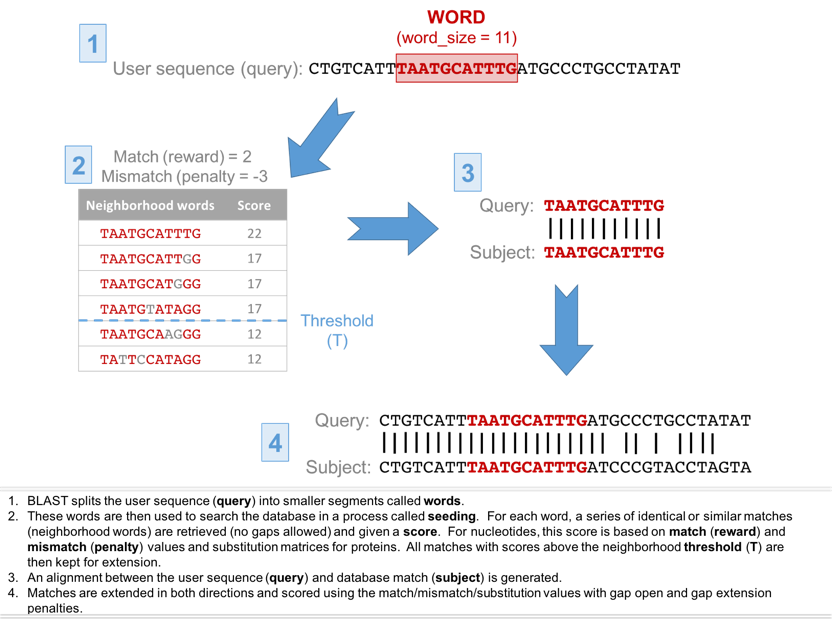
\includegraphics{blast_methods.png}
\caption{How BLAST works}
\end{figure}

    Every BLAST search starts with a query sequence provided by you, the
user. BLAST takes that query sequence and splits it into smaller
fragments called \textbf{\textit{words}}. It then uses these
\textbf{words} to search the database for other sequences that contain
identical or similar, words. This process is called \textbf{seeding}.

Each match or \textbf{hit} is checked to make sure that it meets a
certain threshold or \textbf{score}. The score for each alignment is
calculated using a \textbf{substitution matrix} and, if the score meets
the threshold, the alignment moves forward for \textbf{extension}.
During the extension phase, BLAST will try to increase the length of the
alignment, extending out from either side. Extension will continue until
the \textbf{score} for that alignment falls below a pre-defined
threshold or \textbf{score}. The extended alignment is known as a
\textbf{High-scoring Segment Pair (HSP)}.

So, to recap. The BLAST output for a query sequence is known as the
\textbf{result}. When a sequence that is similar to the query is found
in the database, this is known as a \textbf{hit}. Within the hit there
may be multiple regions of similarity which can be aligned and are known
as a \textbf{HSPs}. Each hit can have multiple \textbf{HSPs} which must
each meet a minimum threshold or \textbf{score}.

    \hypertarget{running-a-simple-blast-search}{%
\subsection{Running a simple BLAST
search}\label{running-a-simple-blast-search}}

All of this sounds great, but it would be easier to understand if we
could see an example, right? Then let's try running one of the simpler
BLAST applications, \textbf{blastn}.



\newpage




First we need to remember the three things we need for any BLAST search:

\begin{itemize}
\tightlist
\item
  A query sequence
\item
  A sequence database
\item
  A BLAST application
\end{itemize}

Now, take another look at the table above, what do we need for a
\textbf{blastn} search?

So, we already have our application, \textbf{blastn} and we have already
generated our nucleotide database \textbf{bacteria\_nucl} in the first
part of the tutorial \href{format_database.ipynb}{here}. All we need now
is our nucleotide query sequence which can be found in
\textbf{example/unknown.fa}.

Let's take a look and check that our query is a nucleotide sequence!

\begin{terminalinput}
\begin{Verbatim}[commandchars=\\\{\}]
\llap{\color{black}\LARGE\faKeyboardO\hspace{1em}} ls example
\end{Verbatim}
\end{terminalinput}

\begin{terminalinput}
\begin{Verbatim}[commandchars=\\\{\}]
\llap{\color{black}\LARGE\faKeyboardO\hspace{1em}} cat example/unknown.fa
\end{Verbatim}
\end{terminalinput}

    So, now we have our three essentials let's run our \textbf{blastn}
search. To look at the parameters available type \textbf{blastn -help}.

\begin{longtable}[]{@{}ll@{}}
\hline
\textbf{Parameter} & \textbf{Meaning}\tabularnewline
\hline
\endhead
\textbf{-task} & Only for blastn and blastp. Defaults to megablast for
blastn.\tabularnewline
\textbf{-query} & The location of the file containing your query
sequence.\tabularnewline
\textbf{-db} & Location and reference (e.g.~bacteria\_nucl) of your
BLAST database\tabularnewline
\textbf{-out} & Location and name of the output file\tabularnewline
\hline
\end{longtable}

The format of the command will be:

\textbf{blastn} \textbf{-task} {[}\textit{task}{]} \textbf{-query}
{[}\textit{input file}{]} \textbf{-db} {[}\textit{database reference}{]}
\textbf{-out} {[}\textit{output file}{]}

As we are not in the same directory as our database, we will need to
tell the program to look in the \textbf{db} folder. We can do this by
putting the location (relative to where we are now) before the reference
e.g. \textbf{db/bacteria/bacteria\_nucl}. You can do the same for the
output file which we want to write to the \textbf{example} folder. It is
normally a good idea to give your output file a descriptive name. Here
we use the program and a generic description of the database being
queried e.g. \textbf{blastn\_bacteria.out}.

Now, let's try and identify our unknown sequence using \textbf{blastn}!

\begin{terminalinput}
\begin{Verbatim}[commandchars=\\\{\}]
\llap{\color{black}\LARGE\faKeyboardO\hspace{1em}} blastn \PYZhy{}task blastn \PYZhy{}query example/unknown.fa \PY{l+s+se}{\PYZbs{}}
            \PYZhy{}db db/bacteria/bacteria\PYZus{}nucl \PY{l+s+se}{\PYZbs{}}
            \PYZhy{}out example/blastn\PYZus{}bacteria.out
\end{Verbatim}
\end{terminalinput}


\newpage



    If this has worked, you should be able to see a new file in the
\textbf{example} directory called \textbf{blastn\_bacteria.out}. To look
at your file, you can open it in a text editor or look at it in the
terminal using the command:

\textbf{less example/blastn\_bacteria.out}

The output can be split into two sections: a summary \textbf{hit} table
and the corresponding \textbf{alignments}. If we were to have multiple
queries, these sections would then be replicated for each query.

Let's take a look at the hit summary\ldots{}

\begin{terminalinput}
\begin{Verbatim}[commandchars=\\\{\}]
\llap{\color{black}\LARGE\faKeyboardO\hspace{1em}} grep \PYZhy{}A \PY{l+m}{10} \PY{l+s+s1}{\PYZsq{}Query=\PYZsq{}} example/blastn\PYZus{}bacteria.out
\end{Verbatim}
\end{terminalinput}

    The hits from the \textbf{bacteria\_nucl} database which match our
unknown sequence are ordered by their \textbf{bit score} from highest to
lowest, the highest representing the \textit{best} hit. This is not the
same as the alignment score that we were discussing earlier. The
\textbf{bit score} is derived from those alignment scores, but is
normalised so that it is possible to compare the alignment scores from
different searches.

In addition to a bit score, each hit is also given an \textbf{E Value}
which represents the number of different alignments that have scores
which are the same or better than a score which is expected to occur by
chance in a database search. Broadly speaking, it is a measure of
confidence. The lower the value the more confident you can be that this
score would not occur by chance.

Let's take a look at the lower end of the table and see how the bit
score and e value differ.

\begin{terminalinput}
\begin{Verbatim}[commandchars=\\\{\}]
\llap{\color{black}\LARGE\faKeyboardO\hspace{1em}} grep \PYZhy{}A \PY{l+m}{5} \PY{l+s+s1}{\PYZsq{}  AY461808.1 \PYZsq{}} example/blastn\PYZus{}bacteria.out
\end{Verbatim}
\end{terminalinput}

    Now let's look at the alignment which corresponds to the \textit{best} hit
(GQ903013.1).

\begin{terminalinput}
\begin{Verbatim}[commandchars=\\\{\}]
\llap{\color{black}\LARGE\faKeyboardO\hspace{1em}} grep \PYZhy{}A \PY{l+m}{18} \PY{l+s+s1}{\PYZsq{}\PYZgt{} GQ903013.1\PYZsq{}} example/blastn\PYZus{}bacteria.out
\end{Verbatim}
\end{terminalinput}

    The alignment gives more detail about this match than the summary table.
Here, the hit is referred to as the \textbf{subject} (or Sbjct). The
alignment gives us details about the orientation of our hit and query
sequences. In this case, the sequences align in the same, forward
direction (Plus/Plus) but this may not always be the case (e.g.~if the
hit was in the reverse orientation Plus/Minus). It also provides
information on the number of exact matches (Identities) and gaps within
our alignment, both of which contribute to the alignment score.

    \textbf{Based on the output of our blastn search, which species do you
think our unknown sequence comes from? What gene might it be?}




\newpage



    \hypertarget{output-formats}{%
\subsection{Output formats}\label{output-formats}}

BLAST results can be written in different formats. If we don't specify
an output format the default is \textbf{pairwise} which contains a
summary hit table and the corresponding alignments as we saw above.
There are several other useful formats which are available using the
\textbf{-outfmt} parameter.

\begin{longtable}[]{@{}ll@{}}
\hline
\textbf{-outfmt value} & ** Description **\tabularnewline
\hline
\endhead
0 & pairwise\tabularnewline
1 & query-anchored showing identities\tabularnewline
2 & query-anchored no identities\tabularnewline
3 & flat query-anchored, show identities\tabularnewline
4 & flat query-anchored, no identities\tabularnewline
5 & XML Blast output\tabularnewline
6 & tabular\tabularnewline
7 & tabular with comment lines\tabularnewline
8 & Text ASN.1\tabularnewline
9 & Binary ASN.1\tabularnewline
10 & Comma-separated values\tabularnewline
11 & BLAST archive format (ASN.1)\tabularnewline
\hline
\end{longtable}

If you don't need to see the alignments, a tabular output is often the
most simple to work with. Let's try adding \textbf{-outfmt 6} to our
command (don't forget to change the output file name!!).

\begin{terminalinput}
\begin{Verbatim}[commandchars=\\\{\}]
\llap{\color{black}\LARGE\faKeyboardO\hspace{1em}} blastn \PYZhy{}task blastn \PYZhy{}query example/unknown.fa \PY{l+s+se}{\PYZbs{}}
            \PYZhy{}db db/bacteria/bacteria\PYZus{}nucl \PY{l+s+se}{\PYZbs{}}
            \PYZhy{}out example/blastn\PYZus{}bacteria\PYZus{}outfmt6.out \PYZhy{}outfmt 6
\end{Verbatim}
\end{terminalinput}

    And take a look at what we've got\ldots{}

\begin{terminalinput}
\begin{Verbatim}[commandchars=\\\{\}]
\llap{\color{black}\LARGE\faKeyboardO\hspace{1em}} head \PYZhy{}10 example/blastn\PYZus{}bacteria\PYZus{}outfmt6.out
\end{Verbatim}
\end{terminalinput}


\newpage



    Our output is now in a tab-delimited format but we have no column names.
By default, these are:

\begin{longtable}[]{@{}ll@{}}
\hline
\textbf{Heading tags} & \textbf{Meaning}\tabularnewline
\hline
\endhead
\textbf{qseqid} & Query identifier/accession\tabularnewline
\textbf{sseqid} & Subject (hit) identifier/accession\tabularnewline
\textbf{pident} & Percentage of identical positions in
alignment\tabularnewline
\textbf{length} & Alignment length\tabularnewline
\textbf{mismatch} & Number of mismatches in alignment\tabularnewline
\textbf{gapopen} & Number of gaps in alignment\tabularnewline
\textbf{qstart} & Start position of alignment in query\tabularnewline
\textbf{qend} & End position of alignment in query\tabularnewline
\textbf{sstart} & Start position of alignment in query\tabularnewline
\textbf{send} & End position of alignment in query\tabularnewline
\textbf{evalue} & E Value\tabularnewline
\textbf{bitscore} & Bit Score\tabularnewline
\hline
\end{longtable}

One useful statistic that we are given when we use the online version of
BLAST is the percentage of our query that has been aligned, also known
as our query coverage. Not to worry, we don't have to manually calculate
this as BLAST has some extra parameters we can use. For more information
try \textbf{blastn -help} and look at the \textbf{Formatting options}
section.

Let's say we don't want to know all of the alignment statistics, how can
we generate a summary which tells us: query id, subject id, query
length, subject length, alignment length, percentage identity, query
coverage, bit score and evalue? Well, we need to specify the
corresponding tags. To do this, we still need to use the
\textbf{-outfmt} parameter but now we put our format identifier (0-11)
followed by the tags for the columns we want to include. The tags should
be separated by a single space with the format identifier and tags all
enclosed in double quotes. Let's give it a try, it will make much more
sense once you see it written out below!

\begin{terminalinput}
\begin{Verbatim}[commandchars=\\\{\}]
\llap{\color{black}\LARGE\faKeyboardO\hspace{1em}} blastn \PYZhy{}task blastn \PYZhy{}query example/unknown.fa \PY{l+s+se}{\PYZbs{}}
            \PYZhy{}db db/bacteria/bacteria\PYZus{}nucl \PY{l+s+se}{\PYZbs{}}
            \PYZhy{}out example/blastn\PYZus{}bacteria\PYZus{}final.out \PY{l+s+se}{\PYZbs{}}
            \PYZhy{}outfmt \PY{l+s+s2}{\PYZdq{}6 qseqid sseqid qlen slen length \PYZbs{}}
        \PY{l+s+s2}{    pident qcovs bitscore evalue\PYZdq{}}
\end{Verbatim}
\end{terminalinput}

    Let's take a look at our output. Remember, the columns are in the same
order as you specified in the command.

\begin{terminalinput}
\begin{Verbatim}[commandchars=\\\{\}]
\llap{\color{black}\LARGE\faKeyboardO\hspace{1em}} head \PYZhy{}10 example/blastn\PYZus{}bacteria\PYZus{}final.out
\end{Verbatim}
\end{terminalinput}

    From this output, you should now be able answer the following questions.

\textbf{What percentage of our query aligns with our top hit?}

\textbf{Is our query sequence the same length as our top hit?}

    \hypertarget{using-different-tasks-to-optimise-parameters}{%
\subsection{Using different tasks to optimise
parameters?}\label{using-different-tasks-to-optimise-parameters}}

    In the last section of the tutorial, you will have noticed that we used
the \textbf{-task} parameter to tell \textbf{blastn} that we want to use
the \textbf{blastn} parameters. But what are these parameters?

If you remember back at the start, we described how BLAST splits your
query sequence into smaller segements called \textbf{words}. The length
of the word is defined by a parameter called \textbf{-word\_size} which
has a default value of 11. Broadly speaking, we can think of this as the
minimum length of the initial alignment which can be found and extended
by BLAST. So,if you have a large database, you can increase the speed of
your search just by increasing word size.

The word size is just one of the parameters which is automatically
changed when you use tasks such as \textbf{megablast}. For
\textbf{megablast}, the word size is increase to a default of 28 and the
cost of opening and extending gaps in the alignment is optimised to find
long, highly similar alignments. This is why \textbf{megablast} is very
efficient and particularly suited to interspecies comparisons.

Let's see if using \textbf{-task megablast} parameters instead of blastn
changes our results. We are going to use the default \textbf{-outfmt 6}
columns this time.

\begin{terminalinput}
\begin{Verbatim}[commandchars=\\\{\}]
\llap{\color{black}\LARGE\faKeyboardO\hspace{1em}} blastn \PYZhy{}task megablast \PYZhy{}query example/unknown.fa \PY{l+s+se}{\PYZbs{}}
            \PYZhy{}db db/bacteria/bacteria\PYZus{}nucl \PY{l+s+se}{\PYZbs{}}
            \PYZhy{}out example/megablast\PYZus{}bacteria\PYZus{}outfmt6.out \PYZhy{}outfmt 6
\end{Verbatim}
\end{terminalinput}

    Let's take a look at our output. Looks pretty similar to the blastn
results, right?

\begin{terminalinput}
\begin{Verbatim}[commandchars=\\\{\}]
\llap{\color{black}\LARGE\faKeyboardO\hspace{1em}} head \PYZhy{}10 example/megablast\PYZus{}bacteria\PYZus{}outfmt6.out
\end{Verbatim}
\end{terminalinput}

    Well, that's not quite true. Let's see how many results we have in both
our blastn and megablast searches.

\begin{terminalinput}
\begin{Verbatim}[commandchars=\\\{\}]
\llap{\color{black}\LARGE\faKeyboardO\hspace{1em}} wc \PYZhy{}l example/blastn\PYZus{}bacteria\PYZus{}outfmt6.out
\end{Verbatim}
\end{terminalinput}

\begin{terminalinput}
\begin{Verbatim}[commandchars=\\\{\}]
\llap{\color{black}\LARGE\faKeyboardO\hspace{1em}} wc \PYZhy{}l example/megablast\PYZus{}bacteria\PYZus{}outfmt6.out
\end{Verbatim}
\end{terminalinput}

    \textbf{Did the blastn and megablast searches produce the same nummber
of hits? Why do you think this is?}\\
(\textit{hint: have a look at the end of the pairwise alignment file and
think about the default megablast word size})

    \hypertarget{searches-using-translated-nucleotide-sequences}{%
\subsection{Searches using translated nucleotide
sequences}\label{searches-using-translated-nucleotide-sequences}}

Sometimes, depending on the biological question (e.g.~don't do this with
primers!), it can be better to perform a BLAST search using a translated
nucleotide query. The simplest explanation is that several codons may
encode the same amino acid (redundancy). So, while there may be
differences between two nucleotide sequences, they may in fact encode
the same amino acid sequence.

So far, we have created our own BLAST database of bacteria sequences and
identified our unknown sequence as TcpC from \textit{Escherichia coli}.
But, is it only found in bacteria?

    \hypertarget{exercise-2}{%
\section{Exercise 2}\label{exercise-2}}

We can't use our bacteria database for this search but we can use what
you learnt in the first part of the tutorial,
\href{format_database.ipynb}{here}, to generate a new database. There
are some sequences provided for you in the db/mammalian folder. Let's
take a look.

\begin{terminalinput}
\begin{Verbatim}[commandchars=\\\{\}]
\llap{\color{black}\LARGE\faKeyboardO\hspace{1em}} ls db/mammalian
\end{Verbatim}
\end{terminalinput}

\begin{terminalinput}
\begin{Verbatim}[commandchars=\\\{\}]
\llap{\color{black}\LARGE\faKeyboardO\hspace{1em}} head db/mammalian/mammalian.fa
\end{Verbatim}
\end{terminalinput}

    \textbf{Using mammalian.fa create a new database which has the output
prefix \textit{mammalian} and can be referenced as \textit{mammalian}.}
(\_hint: you don't need to be in the same folder as your FASTA file to
write your database files there, just prefix the output prefix with the
relative location - e.g.~db/mammalian/mammalian)

\textbf{If our query sequence is nucleotide and we want to search a
protein database, what BLAST application do we need to use?}\\
(\textit{hint: look at the BLAST application table above})

** With example/unknown.fa, run a BLAST search using the application in
your answer above and search the database you have just created. We want
a standard tabulated output file with the following additional columns**
* Full subject title * Query length * Subject length * Percentage query
coverage

\textit{Notice in the previous tabulated output there is only the subject
accession, not the full title/description. For the answer to this
exercise you should look at stitle on the application help page. Also,
you don't need to specify all of the standard output columns, just use
std (e.g. -outfmt ``6 std extra1 extra2\ldots{}''. Remember, as we are
not using either blastn or blastp, we do not need the -task parameter.}

** What is our top hit?\textbf{ } How much of our query sequence is
covered by this alignment?\textbf{ } What is the length of our top hit
and where does the alignment start and finish?**

So, our original question was whether TcpC is only found in bacteria.
The answer is both yes and no. Looking at our answers, we could not find
the whole TcpC protein in the mammalian database (see your answer to for
query coverage). However, we did find a region of similarity in
mammalian toll-like receptors. Biologically, this makes sense as TcpC
and other bacterial protiens contain a region called a TIR domain. These
domains are also found in mammalian innate immune receptors which
include toll-like receptors. There is evidence to suggest that the
similarity between the bacterial TcpC and mammalian immune receptor TIR
domains allow the bacteria to interfere with the host immune system. And
we can see much of this with a simple BLAST!

Well done, you have finished this tutorial! You can
\href{index.ipynb}{return to the index} or revisit the
\href{format_database.ipynb}{previous section}.

The answers to the questions in this tutoial can be found
\href{general_question_and_exercise_answers.ipynb}{here}.


    % Add a bibliography block to the postdoc



\end{document}
